\begin{teamsubmission}{Parse Patrol}{Parse Patrol: Dual-Mode Scientific Parsing Infrastructure via MCP Servers}
\authorsblock{
    Nathan Daelman\textsuperscript{1}\orcidlink{0000-0002-7647-1816},
    Christina Ertural\textsuperscript{2}\orcidlink{0000-0002-7696-5824},
    Rubel Mozumber\textsuperscript{1}\orcidlink{0009-0007-5926-6646},
    Sascha Klawohn\textsuperscript{1}\orcidlink{0000-0003-4850-776X},
    Remya Ann Mathews Kalapurakal\textsuperscript{3} 
}
\affiliationsblock{
    \textsuperscript{1}Humboldt University of Berlin, 10117 Berlin, Germany\\
    \textsuperscript{2}Department of Materials Chemistry, Federal Institute for Materials Research and Testing, 12205 Berlin, Germany\\
    \textsuperscript{3}University of New Hampshire, 03824 Durham, NH, USA
}

\section*{Introduction}

Parsing scientific output files to extract structured data is by its very nature dependent on the input and output specifications.
These specifications may exist at a format level, a schema level, or more abstractly, an ontological one.
Being dependent on both sides, makes parser infrastructure very brittle and labor-intensive to maintain.
This is a frequent issue in materials and chemistry databases and consortia.
Centralizing standards risks breaking existing parsers, while the uncoordinated community approach leaves projects vulnerable to funding cuts.\cite{best_of_atomistic_ml_general} 

Meanwhile, the rise of large language models (LLMs) has opened up new avenues for automating parser development. The complexity in centralizing parser infrastructure has created a natural opportunity for LLM-assisted tooling, since modern models can reason over heterogeneous file formats and dynamically adapt to evolving specifications.
Modern host environments, like IDEs, supply their LLM agents with testing, research, and other development tools.
However, effective use of LLMs requires a reliable interface for connecting models to external tools. MCP provides exactly this mechanism by standardizing how agents discover, invoke, and coordinate such tools.
Anthropic published the Model Context Protocol (MCP)\cite{mcp2024} late last year, defining a general-purpose, host-agnostic interface for such toolkits.
It has since rapidly become the industry standard and is now supported by all major commercial models.
MCP defines a schema in JSON-RPC 2.0 format for communication between agents and a server that exposes several \textit{components}: software \textit{tools}, static and dynamic \textit{resources}, and specially designed system \textit{prompts}. In simple terms, MCP tells an AI agent how to request and use pre-defined tools, resources, and system instructions from a server.

In this work, we present Parse Patrol, an extensible parsing toolkit for AI and human developers alike.
Parse Patrol takes advantage of MCP to integrate various community parsers into a single access point.
It facilitates both (i) a discovery mode, where an agent tests various parsers for converting inputs/instructions to a user-defined schema,
as well as (ii) a direct import mode, where the parsers can be called as modules from code.

\section*{Results}

Automated parser generation faces several pitfalls:
scarce online resources for scientific specifications, model hallucinations outside training data, lengthy test iterations, and unstable software architectures.
Parse Patrol addresses these issues by providing MCP-based access to specialized community parsers and their documentation, enabling wide specification coverage with multiple design options. Because MCP provides a uniform, model-agnostic interface for invoking software tools, individual parsers can be exposed as MCP tools, allowing LLM agents to orchestrate them seamlessly during parser selection, testing, and schema conversion.

Note that MCP does not provide any directives on how to structure tool organization: by default, one just extends the list of tools.
Our first technical innovation is thus to define a \textit{hierarchical protocol} for extending the MCP server.
Each parser is treated as its own MCP server.
This facilitates testing, as the developer can instantiate just that single server.
All MCP components are then automatically registered to the central, user-facing server.
This server predominantly adds its own engineered prompts for deploying tests or production.
Specifications are provided directly in the chat or as a separate file.
Test cases can be downloaded via database MCP servers.

While MCP enables interactive testing or one-off usage, production and en masse processing require actual code.
Without explicit prompting, agents generate parsers from scratch rather than using MCP servers, relying on training data or attempting to locate MCP installation paths.
Therefore, we provide the MCP tools, normally reserved for the discovery phase, as code modules too.
As modules, we also guarantee their installation setup, further offloading a burden of the agent.

Even so, the agent will not automatically pick up on these modules.
We attribute this behavior to the underlying models not having been trained on a MCP/module hybrid.
Our solution is two-pronged: we provide instructions in the relevant prompts to use the modules.
Each parser server exposes its module path and how to call it as a resource.
These are then compiled into a list of resources at the central server.

Providing such a common solution that is both a MCP server and a module is challenging.
Each framework has different requirements and is distributed via different channels: \href{https://github.com/modelcontextprotocol/servers}{MCP Registry}\cite{mcp2024registry} and \href{https://pypi.org/}{PyPi}\cite{pypi}, respectively, for example.
Our second innovation, then, is the design of a \textit{dual mode} (cf. Fig.\ref{fig:parse-patrol}) that facilitates the free combination of either feature.
To the best of the authors' knowledge, no other such framework exists that bridges the divide between AI experimentation and production integration.

\begin{figure}[h]
    \centering
    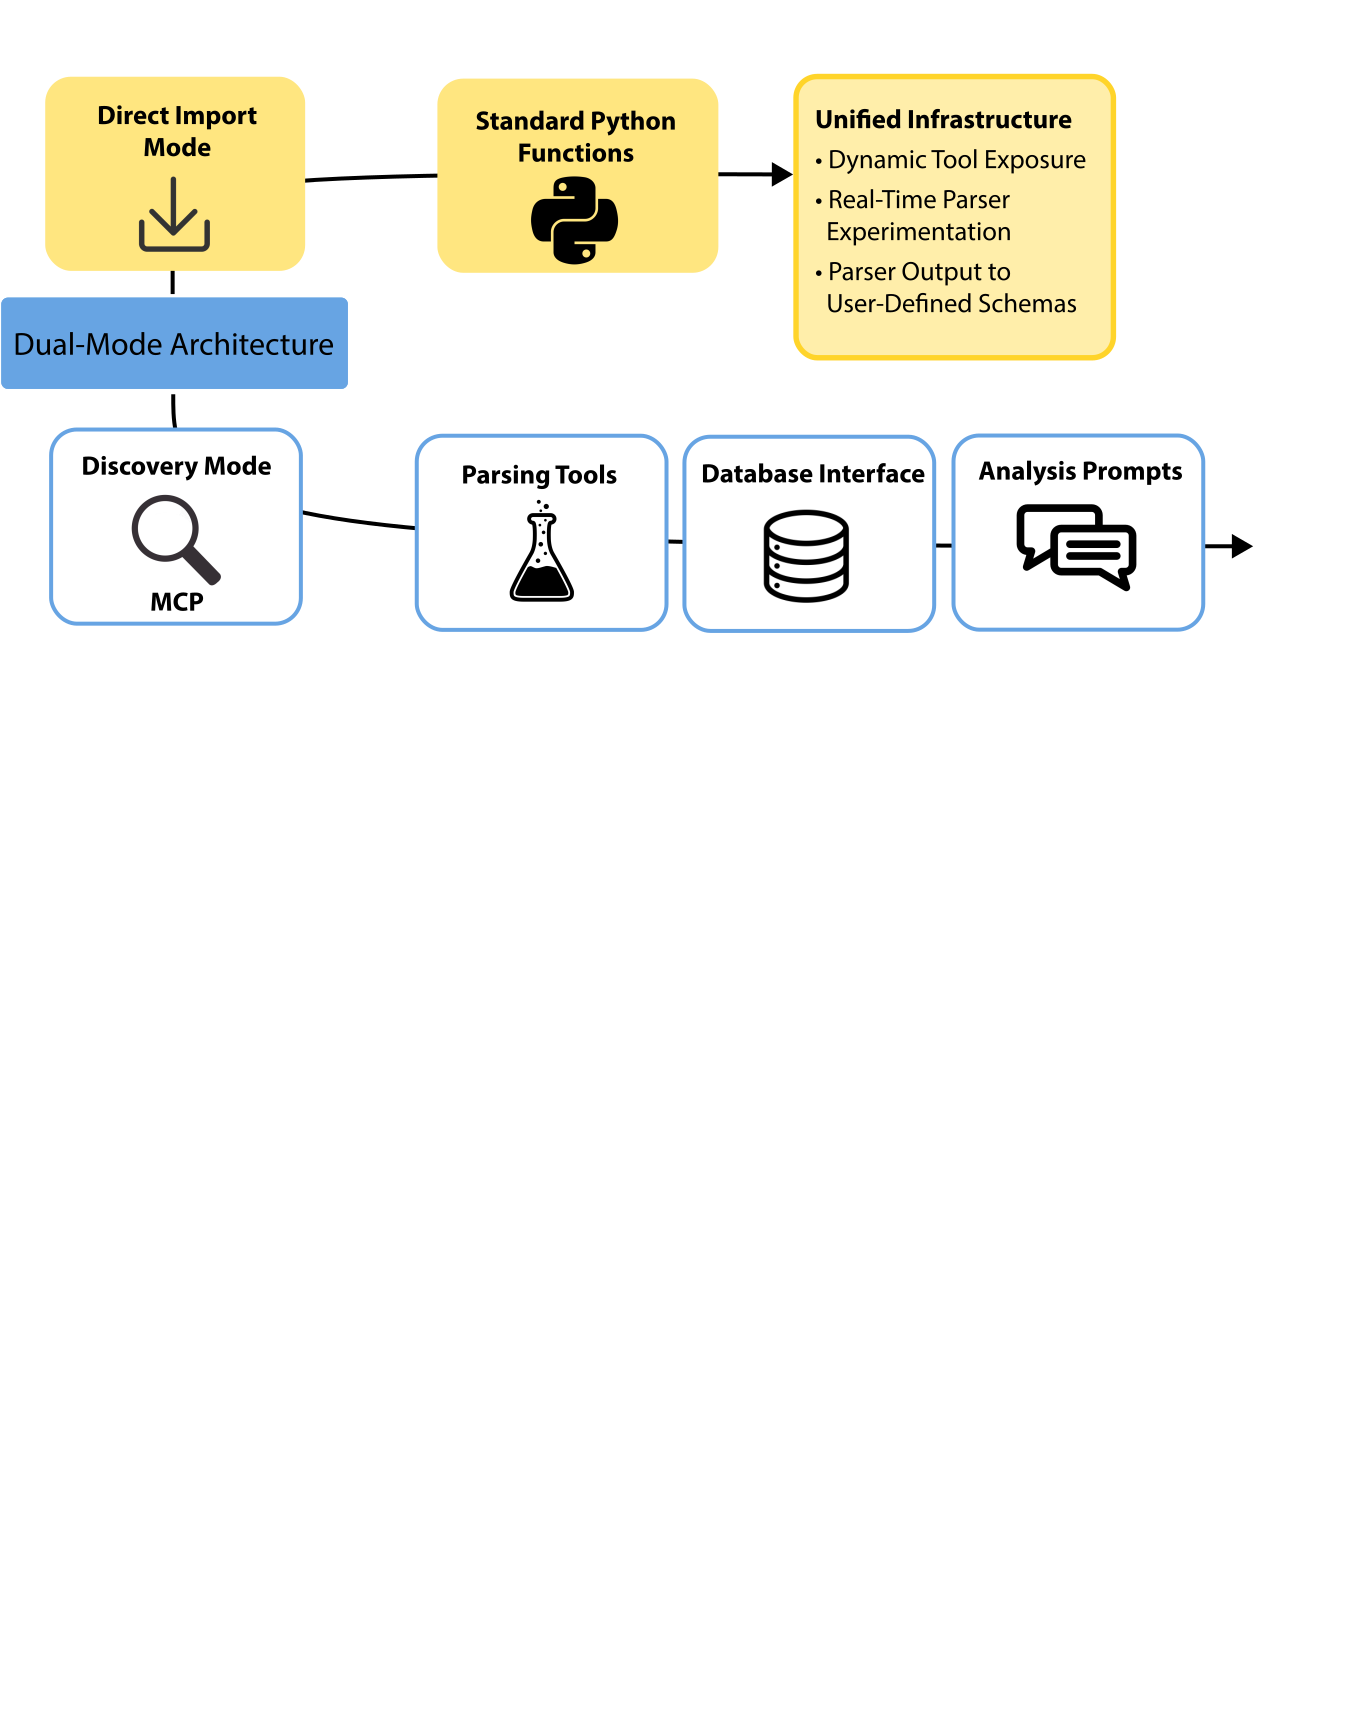
\includegraphics[width=0.8\linewidth]{figures/parse-patrol.png}
    \captionsetup{width=\linewidth}
    \caption{
    Schematic depiction of the \textit{dual-mode} design in Parse Patrol.
    \textbf{Lower branch:} Discovery mode provides a single MCP interface to several parser and database servers.
    The central server further exposes pre-engineered prompts for the suggested use case.
    Most hosts provide shortcuts to these prompts.
    \textbf{Upper branch:} Direct Import mode exposes the same MCP components as Python modules for friction-less switching from testing to production.
    Both branches are unified under a unified architecture.
    }
    \label{fig:parse-patrol}
\end{figure}

\section*{Future Work}

At the time of writing, the repository is seeing active development.
Given the well-defined objective of providing a computational parsers toolkit, future extensions are not excluded.
This project is under consideration for incorporation into NOMAD parser suite\cite{nomad_lab,draxl2019nomad}.

\section*{Open Source Materials}

The open source code is available on GitHub: \github{https://github.com/ndaelman-hu/parse-patrol}. 
A demo video is available on YouTube: \youtube{https://www.youtube.com/watch?v=fSAyi5ubkR0}.

\section*{Author Contributions}

\textbf{N.D.}: Conceptualization, Software, Original Code Draft, Visualization - Writing of Documentation and Manuscript, Editing
\textbf{C.E.}: Conceptualization Revision, Software, Visualization, Video Editing, Writing - Original Manuscript Text Draft, Figure, Editing
\textbf{R.M.}: Implementation asynchronous servers, Extension Testing Infrastructure - Conceptualization Revision, Proof-read Manuscript
\textbf{S.K.}: Extend Parser Servers - Proof-read Manuscript
\textbf{R.A.M.K.}: Testing of Setup, Trial new Parsers - Proof-read Manuscript

\section*{Acknowledgements}
This work was supported by the NFDI consortium FAIRmat - Deutsche Forschungsgemeinschaft (DFG) - Project 460197019.

\end{teamsubmission}
